% =========================================================================== %
% TeX input file: "SDK - Editor - Icons"
%
% WARNING: this tex file does not compile standalone, it needs to be embedded
% in a master tex document (e.g. Introduction.tex)
% =========================================================================== %

The Icons Editor allows to visualize the Icons defined in the \java{Icons} class. 

\subsubsection*{Open the Icons Editor}

Expand the \node{shared} node of the Eclipse Scout project in the \scoutExplorerView and select the \folder{Icons} folder. Click the link \textsc{Open Icons Editor} in the \scoutPropView. 

\subsubsection*{Description of the Icons Editor}

\begin{figure}
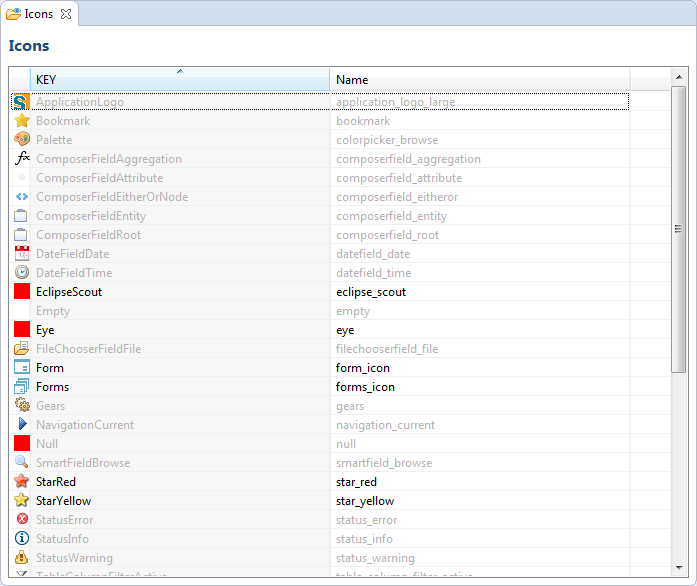
\includegraphics[width=14cm]{sdk_editor_icons.png}
\caption{Screenshot of the Icons Editor}
\figlabel{sdk_editor_icons}
\end{figure}

The editor shown on in \figref{sdk_editor_icons} contains a table displaying the constants defined in the Icons class. For each constant (corresponding to an image), the icon, the key and the name are displayed.

Images defined in the parent class are displayed in gray (they represents the images inherited from a parent class). Images defined in this class are displayed in black.


% =========================================================================== %
% EOF TeX input file
% =========================================================================== %
